\documentclass[12pt, titlepage]{article}

\usepackage{booktabs}
\usepackage{tabularx}
\usepackage{hyperref}
\usepackage{float}
\usepackage{graphicx}
\usepackage{amsmath, mathtools}
\hypersetup{
    colorlinks,
    citecolor=black,
    filecolor=black,
    linkcolor=red,
    urlcolor=blue
}
\usepackage[round]{natbib}

\input{../Comments}
%% Common Parts

\newcommand{\progname}{Baja Dynamics} % PUT YOUR PROGRAM NAME HERE
\newcommand{\authname}{Team \#17, Team Name
\\ Grace McKenna
\\ Travis Wing
\\ Cameron Dunn
\\ Kai Arseneau} % AUTHOR NAMES                  

\usepackage{hyperref}
    \hypersetup{colorlinks=true, linkcolor=blue, citecolor=blue, filecolor=blue,
                urlcolor=blue, unicode=false}
    \urlstyle{same}
                                


\begin{document}

\title{Verification and Validation Report: \progname} 
\author{\authname}
\date{\today}
	
\maketitle

\pagenumbering{roman}

\section{Revision History}

\begin{tabularx}{\textwidth}{p{3cm}p{2cm}X}
\toprule {\bf Date} & {\bf Version} & {\bf Notes}\\
\midrule
Date 1 & 1.0 & Notes\\
Date 2 & 1.1 & Notes\\
\bottomrule
\end{tabularx}

~\newpage

\section{Symbols, Abbreviations and Acronyms}

\renewcommand{\arraystretch}{1.2}
\begin{tabular}{l l} 
  \toprule		
  \textbf{symbol} & \textbf{description}\\
  \midrule 
  T & Test\\
  \bottomrule
\end{tabular}\\

\wss{symbols, abbreviations or acronyms -- you can reference the SRS tables if needed}

\newpage

\tableofcontents

\listoftables %if appropriate

\listoffigures %if appropriate

\newpage

\pagenumbering{arabic}

This document ...

\section{Functional Requirements Evaluation}

\subsection{Simulation Model}

\subsubsection{Position}
\begin{enumerate}
\item{\textbf{Position test-1}: Graphical validation}\\

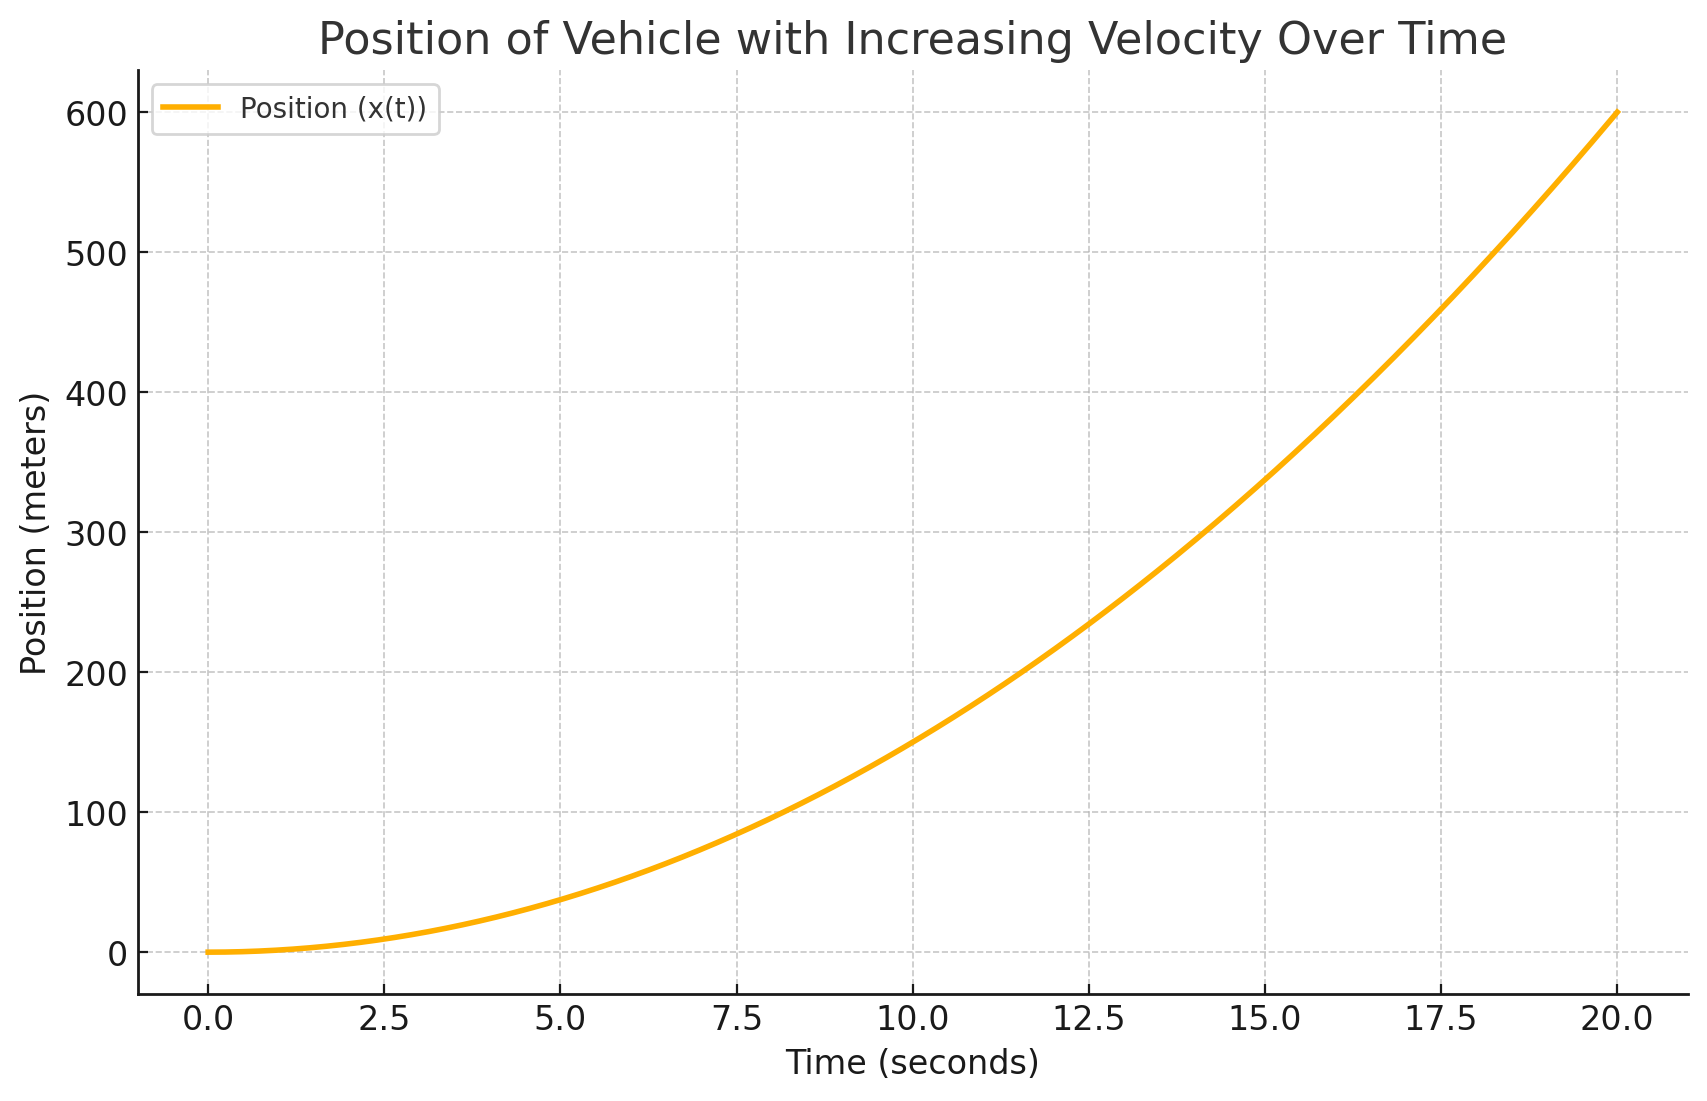
\includegraphics[width=0.5\textwidth]{theoretical-figures/position.png}
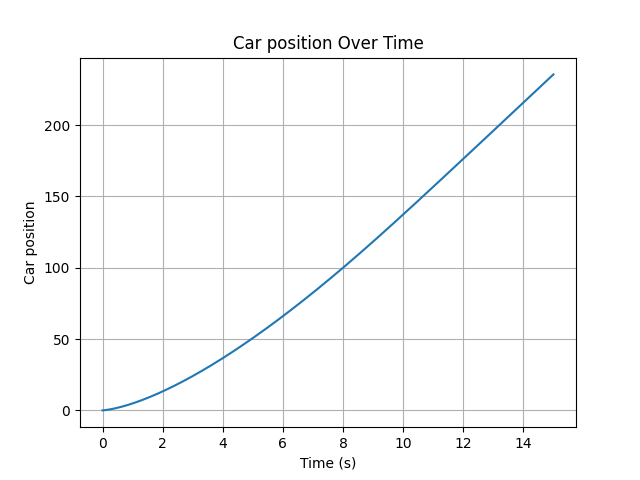
\includegraphics[width=0.5\textwidth]{simulation-figures/car_position.png}

As seen above, the simulation output for the position of the car is consistent with the theoretical model. The larger initial slope can be attributed to an initial velocity, which is required due to \textbf{A9: No belt slippage} in \href{https://github.com/gr812b/CVT-Simulator/blob/develop/docs/SRS/SRS.pdf}{SRS}.

\item{\textbf{Position test-2}: MSE against experimental data}\\
See the \href{https://github.com/gr812b/CVT-Simulator/blob/develop/docs/VnVExtra/VnVExtra.pdf}{VnV Extra}.

\end{enumerate}

\subsubsection{Velocity}
\begin{enumerate}
\item{\textbf{Velocity test-1}: Graphical validation}\\

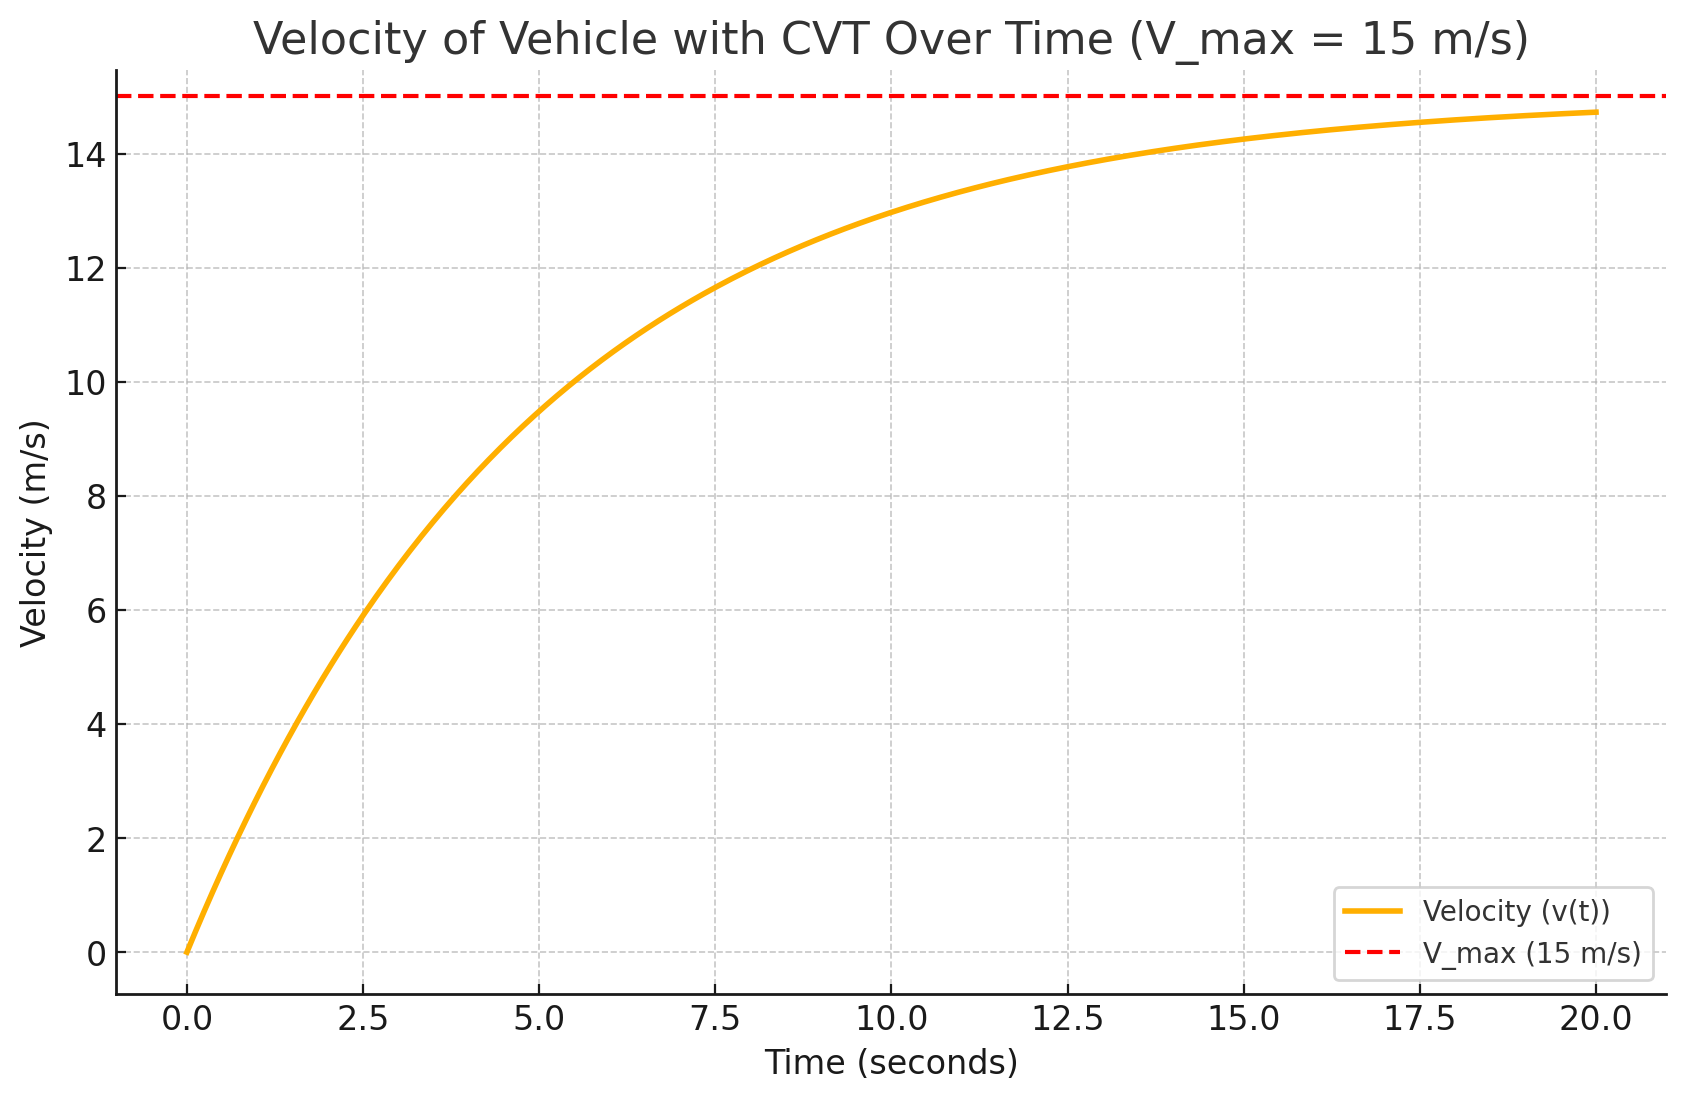
\includegraphics[width=0.4\textwidth]{theoretical-figures/velocity.png}
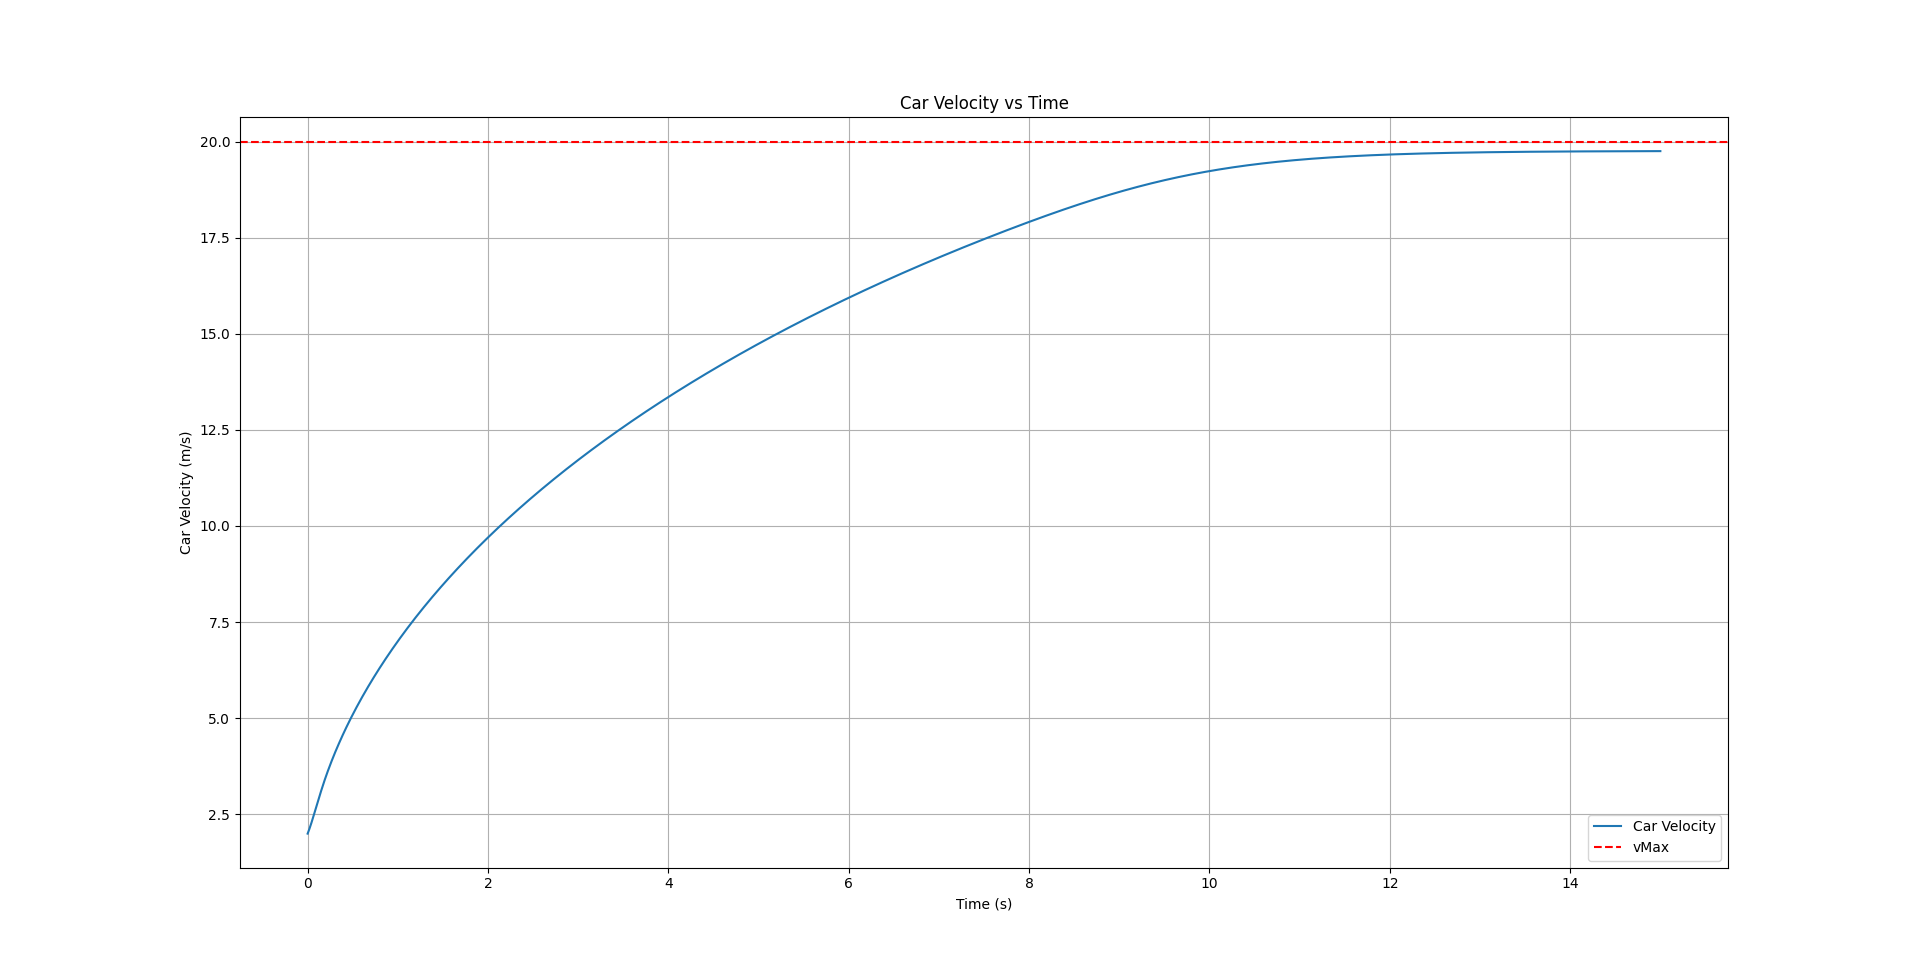
\includegraphics[width=0.5\textwidth]{simulation-figures/car_velocity.png}

As seen above, the simulation output for the velocity of the car is consistent with the theoretical model. The $v_\text{max}$ may be subject to changes according to approximations when calculating air resistance.

\item{\textbf{Velocity test-2}: MSE against experimental data}\\
See the \href{https://github.com/gr812b/CVT-Simulator/blob/develop/docs/VnVExtra/VnVExtra.pdf}{VnV Extra}.

\end{enumerate}

\subsubsection{Acceleration}
\begin{enumerate}
\item{\textbf{Acceleration test-1}: Graphical validation}\\

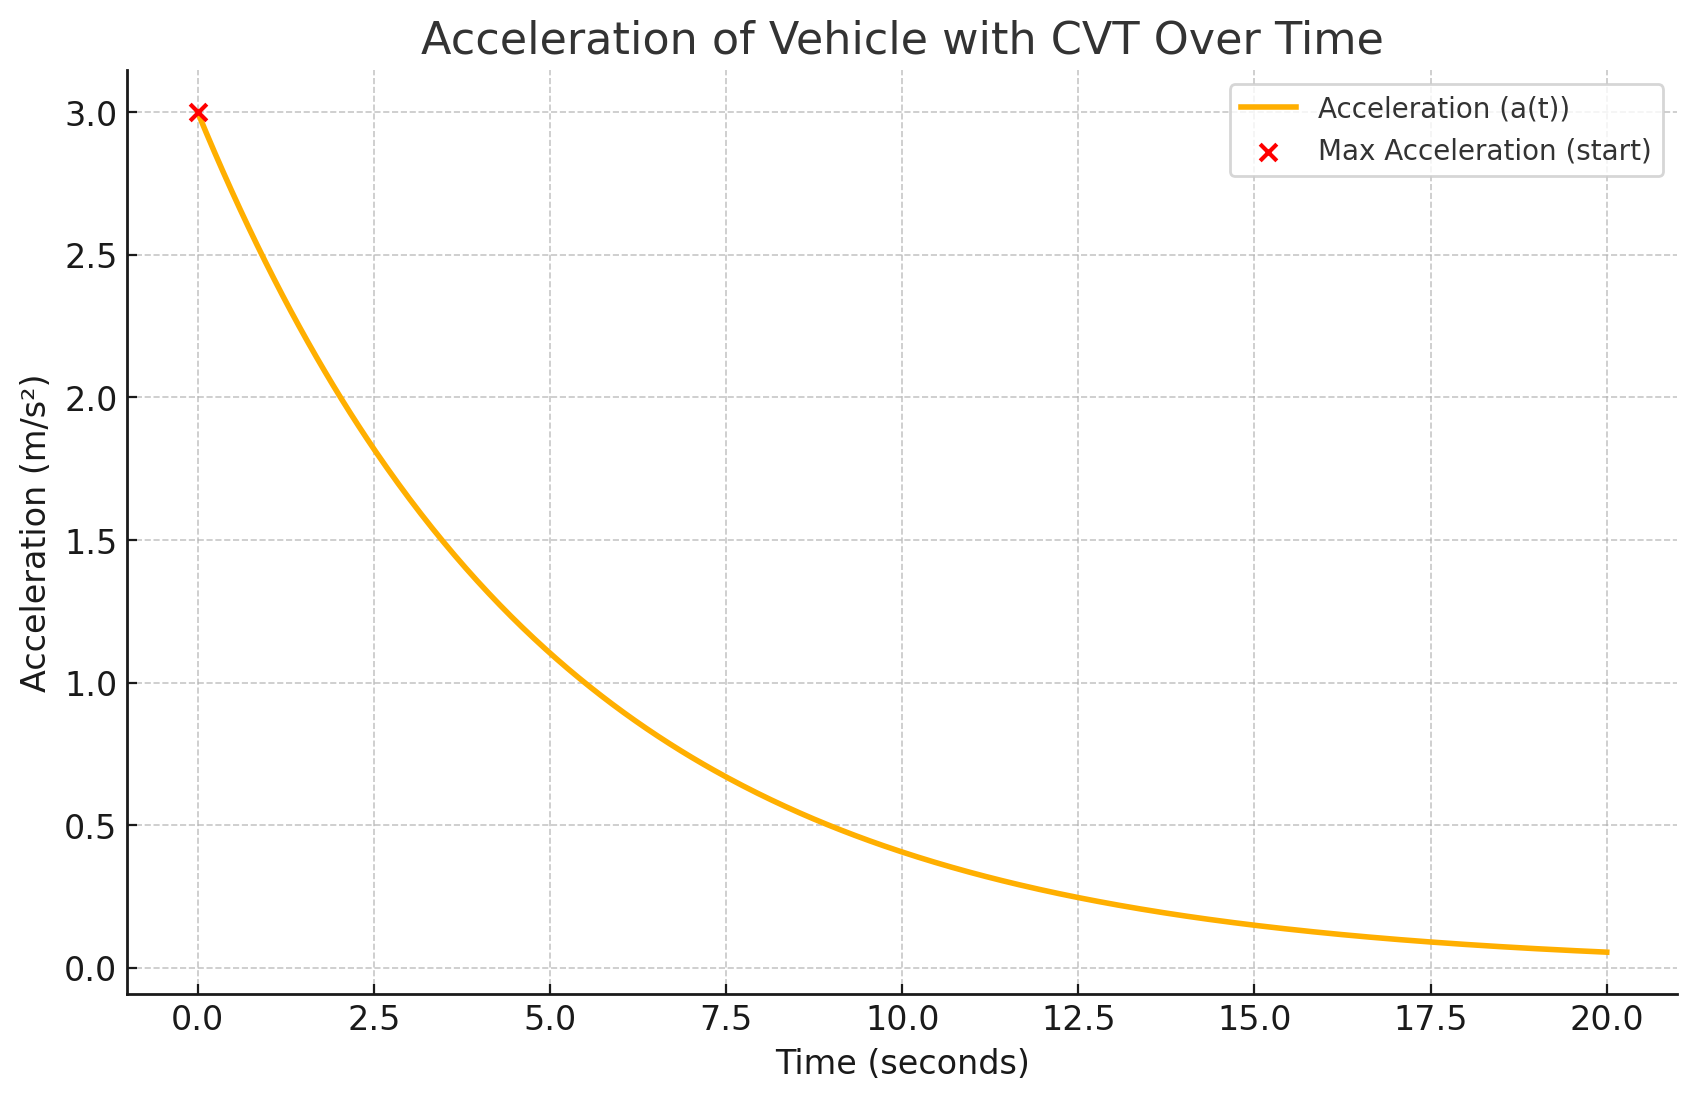
\includegraphics[width=0.4\textwidth]{theoretical-figures/acceleration.png}
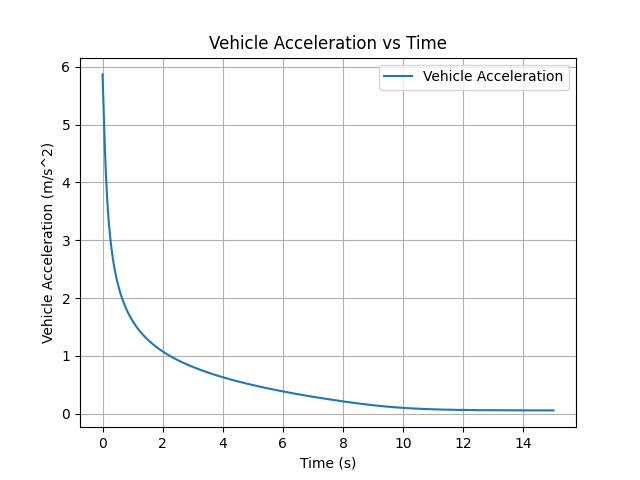
\includegraphics[width=0.5\textwidth]{simulation-figures/vehicle_acceleration.png}

The vehicle's acceleration matches the general shape of the theoretical model. The slope of the theoretical model was simply an estimate, meant to capture the shape of the graph, and so is a bit less accurate than the other graphs. Despite this, both share a common structure and follow expected trends.
\item{\textbf{Acceleration test-2}: MSE against experimental data}\\
See the \href{https://github.com/gr812b/CVT-Simulator/blob/develop/docs/VnVExtra/VnVExtra.pdf}{VnV Extra}.

\end{enumerate}

\subsubsection{Clamping Forces}
\begin{enumerate}
\item{\textbf{Clamping forces test-1}: Graphical validation}\\

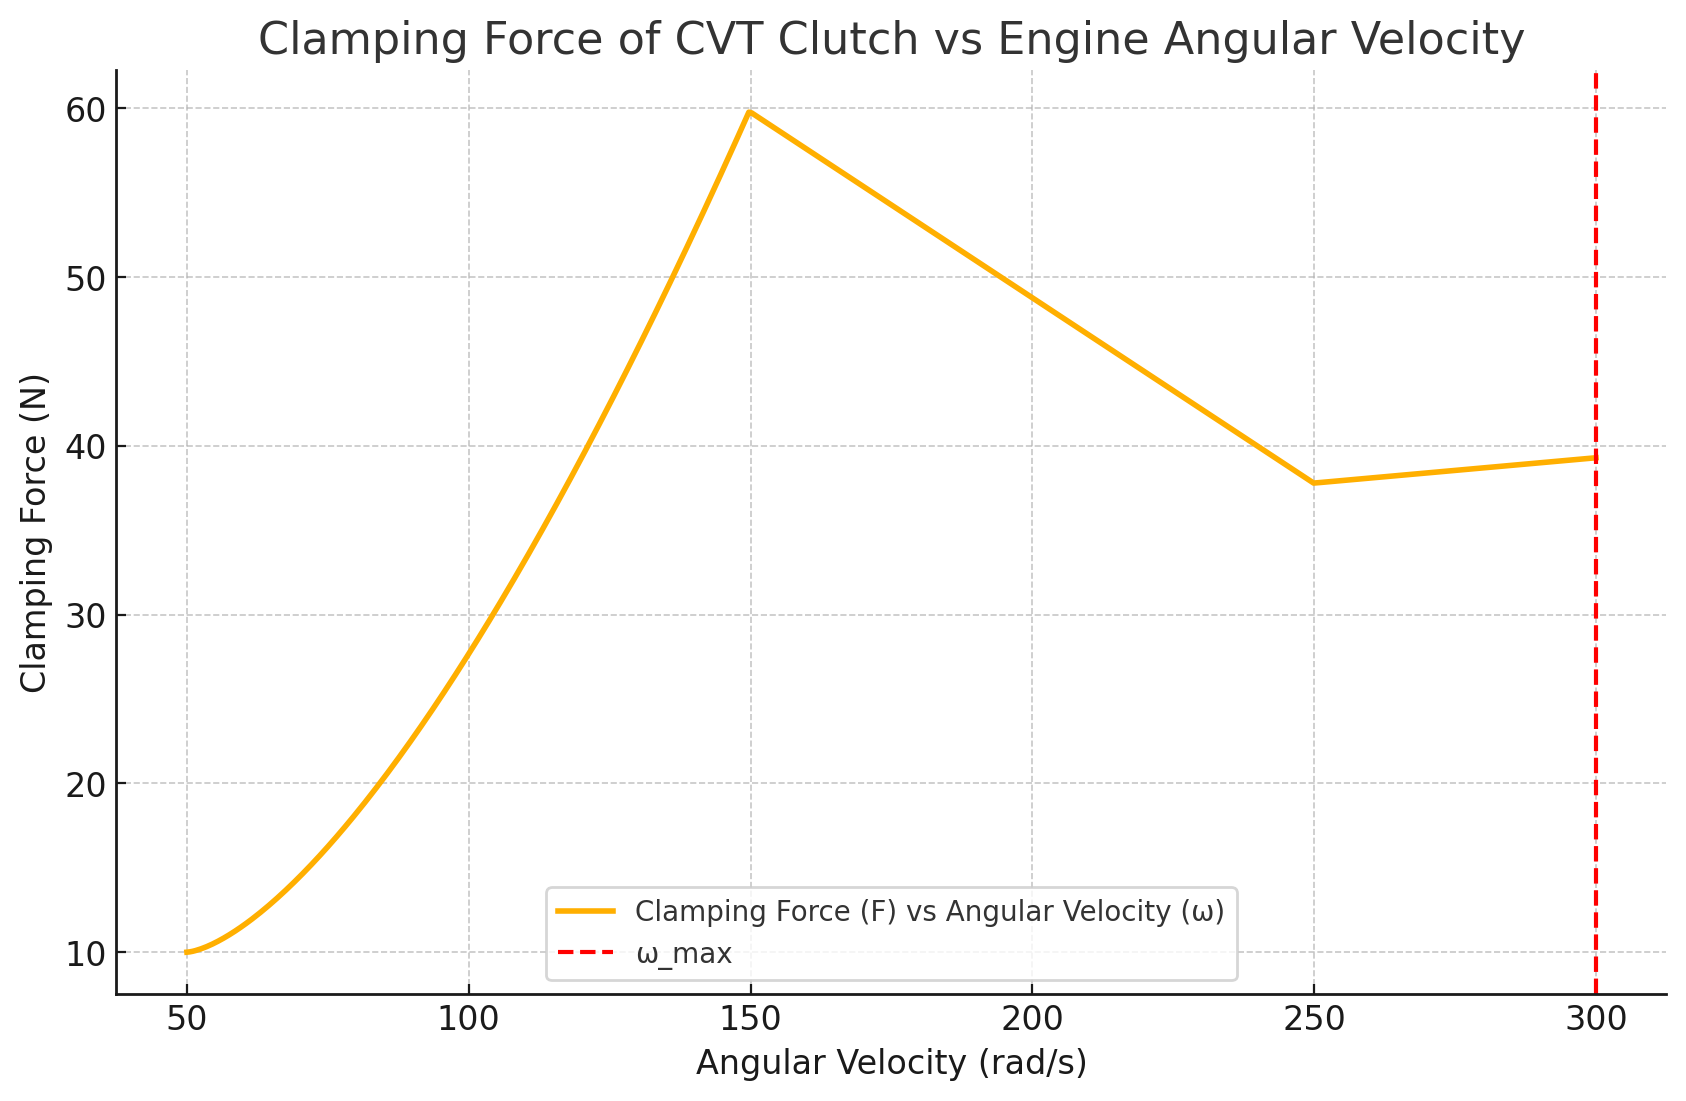
\includegraphics[width=0.4\textwidth]{theoretical-figures/clamp_force.png}
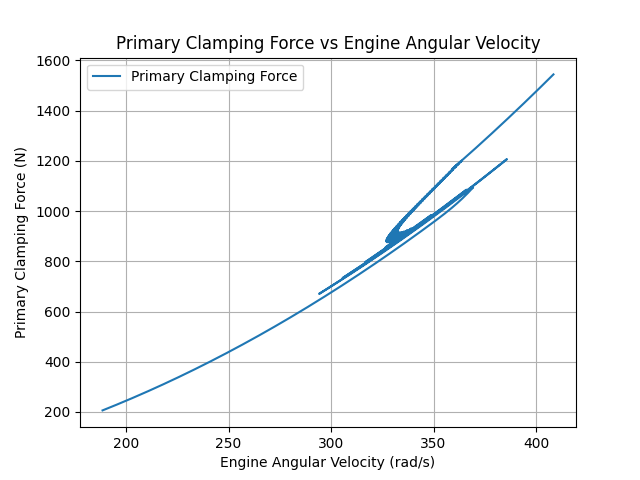
\includegraphics[width=0.5\textwidth]{simulation-figures/primary_clamping.png}

The shape of both graphs above do not match. While the expected result is an initial sharp increase, which then leads to a steady decrease, followed finally by an increase at the end, here we can see what is effectively exclusively an increase with some oscillations. This difference can be explained thanks to two factors.

First, the oscillations arise due to \textbf{A9: No belt slippage} in \href{https://github.com/gr812b/CVT-Simulator/blob/develop/docs/SRS/SRS.pdf}{SRS}, which result in an underdamped system. 

Secondly, the exclusive increase is due to a poor representation of the complex ramp geometry. While in the real world, we know the ramp begins linear, then transitions to a gentle curve that gives us the decrease in force as we shift, the simulation represents it as a linear line. This causes a more strict rising of the force at each corresponding angular velocity of the engine.

The impact this has on the system is quite miniscule. As long as the initla clamping forces which drive the shifting behaviour are correct, the majority of the system should behave as expected. Since our shifting occurs at one specific angular velocity, we need not worry about some of the extremeties being too far off. Further, the real world downsides of having an ever-increasing clamping force would be an excess of heat, which is ignored in our simulation via \textbf{A5: Ignore Wear and Tear} and \textbf{A1: No Material Variations by Temperature} in \href{https://github.com/gr812b/CVT-Simulator/blob/develop/docs/SRS/SRS.pdf}{SRS}

\end{enumerate}

\subsubsection{Shift}
\begin{enumerate}
\item{\textbf{Shift test-1}: Graphical validation 1}\\

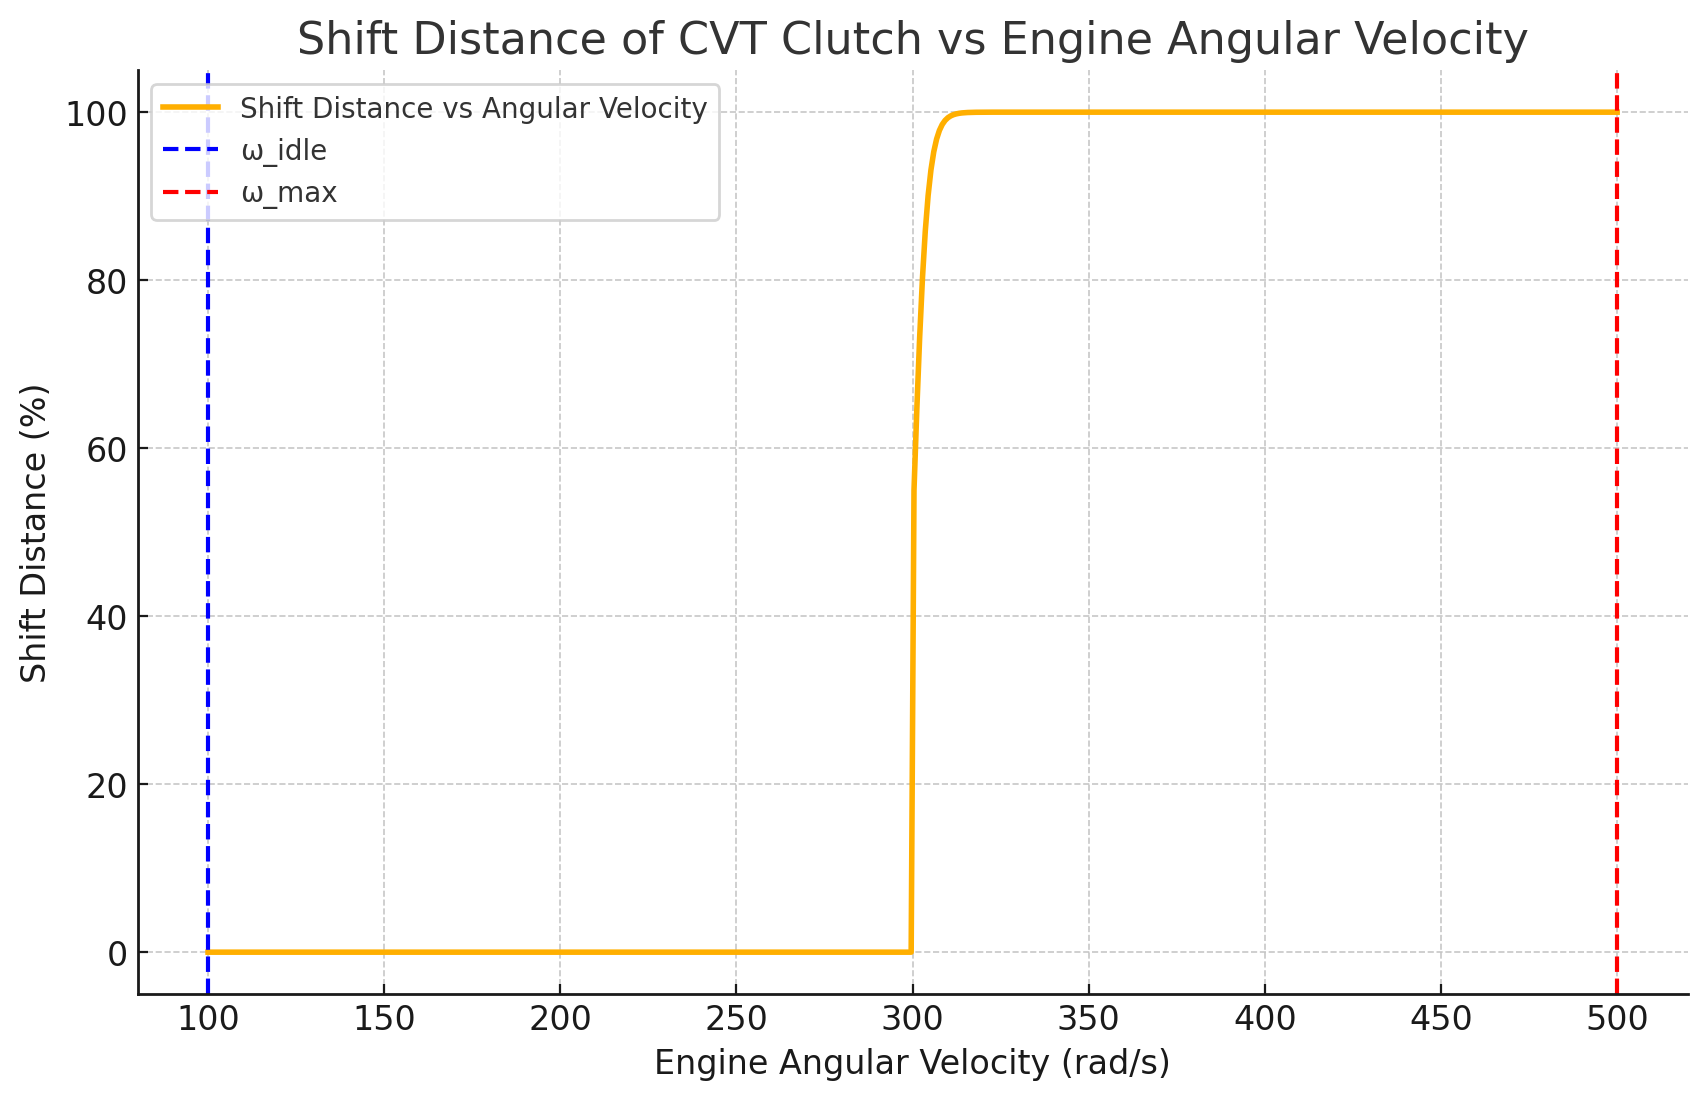
\includegraphics[width=0.5\textwidth]{theoretical-figures/shift_vs_engine.png}
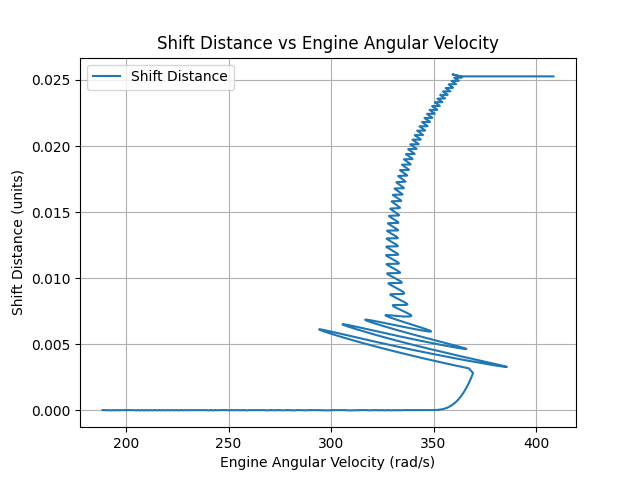
\includegraphics[width=0.5\textwidth]{simulation-figures/shift_distance_vs_engine_velocity.png}
We can see the graphs are quite close in shape. Some key differences include:
\begin{itemize}
  \item the magnitude at which we shift, which is variable and can be altered based on the input parameters.
  \item The oscillations in the simulation are due to \textbf{A9: No belt slippage} in \href{https://github.com/gr812b/CVT-Simulator/blob/develop/docs/SRS/SRS.pdf}{SRS}, which cause an underdamped system.
  \item The slight slope within the simulation. This is due to the poor ramp representation alongside other input parameters. Will be discussed more in Shift test-3.
\end{itemize}


\item{\textbf{Shift test-2}: MSE against experimental data 1}\\
See the \href{https://github.com/gr812b/CVT-Simulator/blob/develop/docs/VnVExtra/VnVExtra.pdf}{VnV Extra}.

\item{\textbf{Shift test-3}: Graphical validation 2}\\

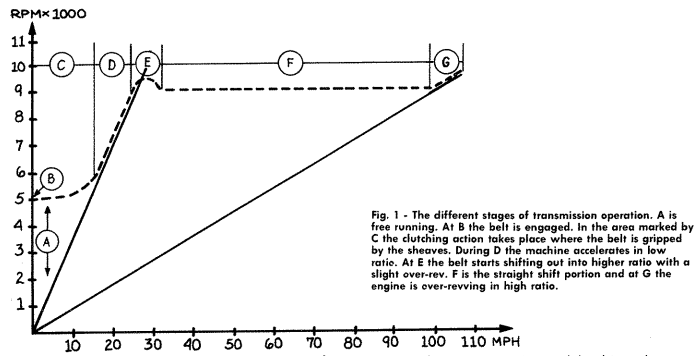
\includegraphics[width=0.5\textwidth]{theoretical-figures/shift_curve.png}
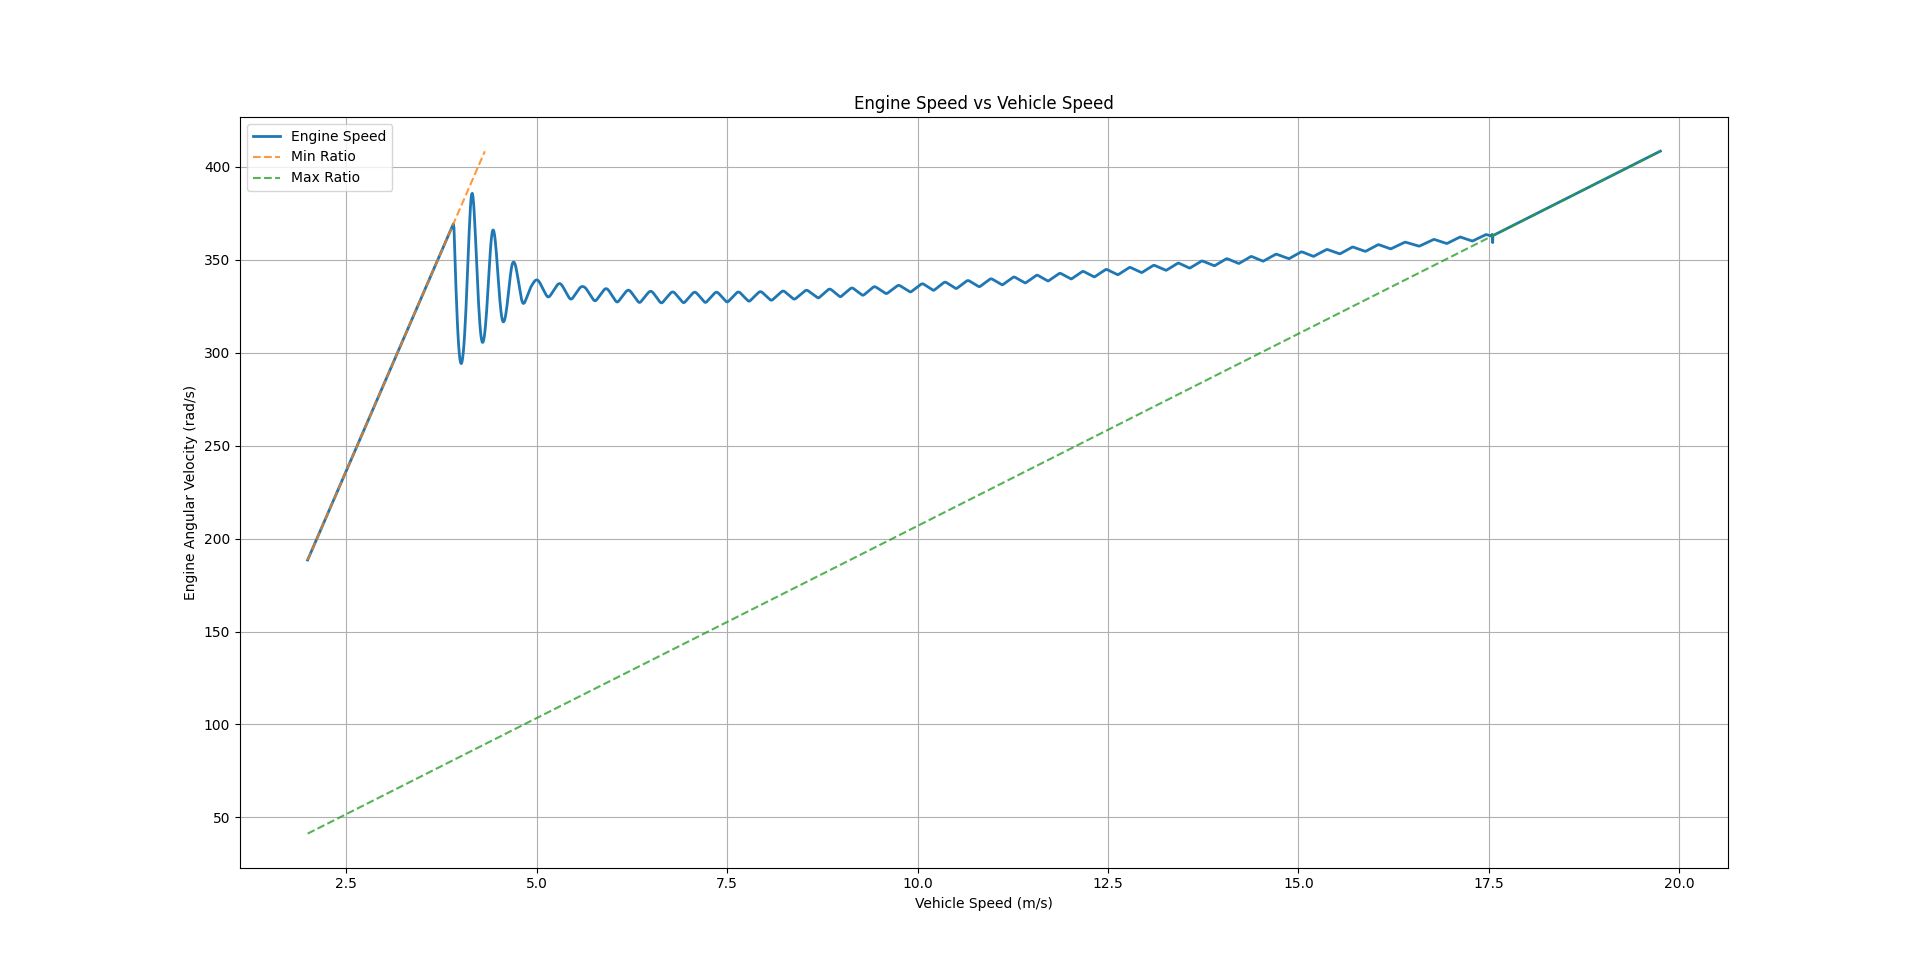
\includegraphics[width=0.5\textwidth]{simulation-figures/shift_curve.png}

The shift curve seen here shows much about the system, as so we will go over each section within the graph.
\begin{itemize}
\item{Phase A to C:} Due to \textbf{A9: No belt slippage} in \href{https://github.com/gr812b/CVT-Simulator/blob/develop/docs/SRS/SRS.pdf}{SRS}, it is unreasonable to omdel these portions. Were the engine tied to the vehicle's tired without slip, at low velocities the engine would be spinning lowering than it is capable of maintaining, and would thus kill the system. The solution in our simulation is to skip this portion, beginning at an initial velocity of around 3.5m/s.
\item {Phase D and E:} This portion is modelled quite well. Here we see the vehicle and engine gaining speed at the low-ratio gear. We also see a slight overshoot thanks to the momentum of the system.
\item {Phase F:} This is the shifting phase, which has the bulk of the calculations in our system affecting. Overall, a similar shape is reflected in both, with a mostly horizontal line. The slight slope in the simulation arises as we begin to shift too slowly, which allows the engine to gain speed. This can be attributed to several factors, but the most prominent is the poor ramp representation. The ramp is modelled as a linear line, which causes the system to shift too slowly. This is a minor issue, as the system still shifts at the correct time, but the speed at which it shifts is too slow.
\item {Phase G:} In the final phase, we see the system accelerate at the high-ratio gear. Both graphs match exactly in this portion.
\end{itemize}

\item{\textbf{Shift test-2}: MSE against experimental data 2}\\

See the \href{https://github.com/gr812b/CVT-Simulator/blob/develop/docs/VnVExtra/VnVExtra.pdf}{VnV Extra}.

\end{enumerate}

\subsubsection{Engine Dynamics}
\begin{enumerate}
\item{\textbf{Engine test-1}: Graphical validation}\\

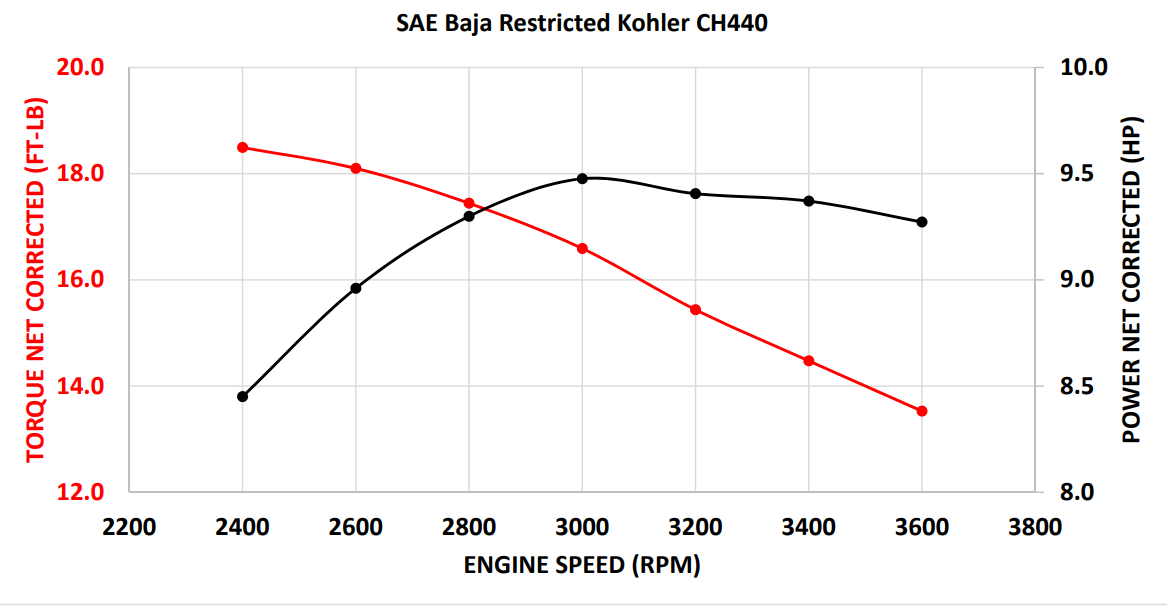
\includegraphics[width=0.4\textwidth]{theoretical-figures/engine.png}
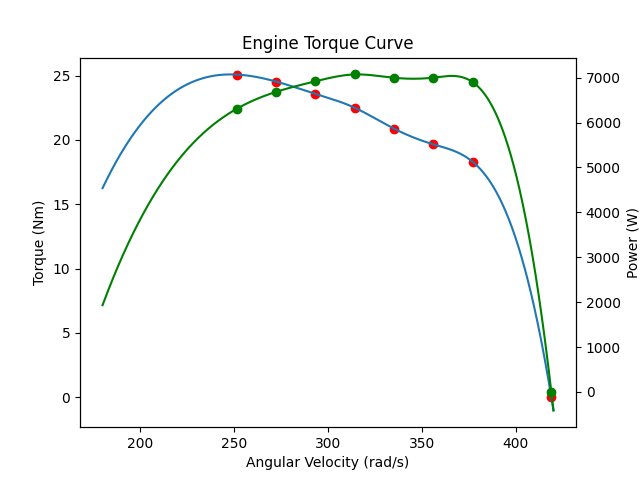
\includegraphics[width=0.5\textwidth]{simulation-figures/engine_specs.png}

As seen in these two graphics, all points within the theoretical figures are represented exactly in the simulation. The only addition is seen via a point at our max engine RPM of 4000, which is limited by the official Baja SAE rules [LINK HERE]. The produced torque at this point drops to 0, as a restrictor plate ensures no additional power may be produced beyond this speed.

\end{enumerate}

\subsection{User Interface}
\begin{enumerate}
\item{\textbf{User Interface test-1}: Input Parameters}\\
The input parameters are loaded with the default values. The user can adjust the parameters and the simulation will run with the new parameters. The user can also save the parameters to a file and load them back in. The user can also export the simulation data to a file.
\item{\textbf{User Interface test-2}: User Interface}\\
When the user launches the application they are presented with a main menu. From here they can navigate to the simulation screen where they can adjust the parameters and run the simulation
\item{\textbf{User Interface test-3}: Viewing Data Outputs}\\
The user can view the data outputs in the simulation screen. The user has an option to view the data displayed in a graph format and the user can see the position, velocity, acceleration, and shift distance of the car over time.
\item{\textbf{User Interface test-4}: Saving and Exporting Data}\\
From the results screen the user can save the parameters inputted to the simulation to a file. The user can also export the simulation data to a csv file for further analysis.
\end{enumerate}

\section{Nonfunctional Requirements Evaluation}

This section will cover the evaluation of the Nonfunctional Requirements. 

\subsection{Accuracy}

The accuracy test involves the outputs of the following Functional Test cases: \textbf{Position test-2}, \textbf{Velocity test-2}, \textbf{Acceleration test-2}, \textbf{Shift test-2} and \textbf{Shift test-4}. 
The following Accuracy test is to be completed in the VNV EXTRA. 

\begin{enumerate}
  \item{\textbf{Accuracy test-1}:}
  This test will take the outputted data of above listed functional tests. 
  As each of these tests will output the MSE, each MSE should fall within 0.2 of 0.
  A range within 0.2 of 0 for each MSE outputted will indicate an accurate system. 
  
\end{enumerate}

		
\subsection{Usability}
The Usability/Understandability survey remains in progress at this time and results will be discussed in the \href{file:../UsabilityReport/UsabilityReport.pdf}{Usability Report}. 
Therefore, Usability test-1 and Usability test-2 have not been fully completed yet, however as they are in progress these tests will be completed as future work. 

\begin{enumerate}
\item{\textbf{Usability test-1}: Navigating Main Interface}\\
Survey question: On a scale of 1-5 with 1 being extremely difficult and 5 being extremely easy, how easy was it to navigate the main interface? 
\item{\textbf{Usability test-2}: Use of Most Common Features}\\
Survey question: For the following main features: Inputting parameters, Adjusting parameters, Viewing data outputs, Saving and exporting data. 
Rate each feature on a scale of 1-5 with 1 being extremely difficult and 5 being extremely easy
\end{enumerate}

\subsection{Maintainability}
The maintainability tests are designed to test how maintainable the system is given likely future changes.
\begin{enumerate}
\item{\textbf{Maintainability test-1}}\\
This test was manually completed where the amount of time and number of lines of code
will be recorded when implementing the changes that correspond to the 2023 CVT configuration. 
Implementation of the 2023 CVT parameters takes at most 20 minutes with modifications to appropriately 26 lines of code in the \texttt{car\_specs.py}.
Thus, the system is easily maintainability and the number of lines modified and time taken is minimal given a total change in parameters of the CVT. 
\end{enumerate}
\subsection{Verifiability}
The tests for verifiability involve completing \textbf{Position test-1}, \textbf{Velocity test-1}, \textbf{Acceleration test-1}, \textbf{Shift test-1} and \textbf{Shift test-3}.
For each of the above tests, they will be run 30 times with the same input parameters to verify that the output produced is the same each time. 


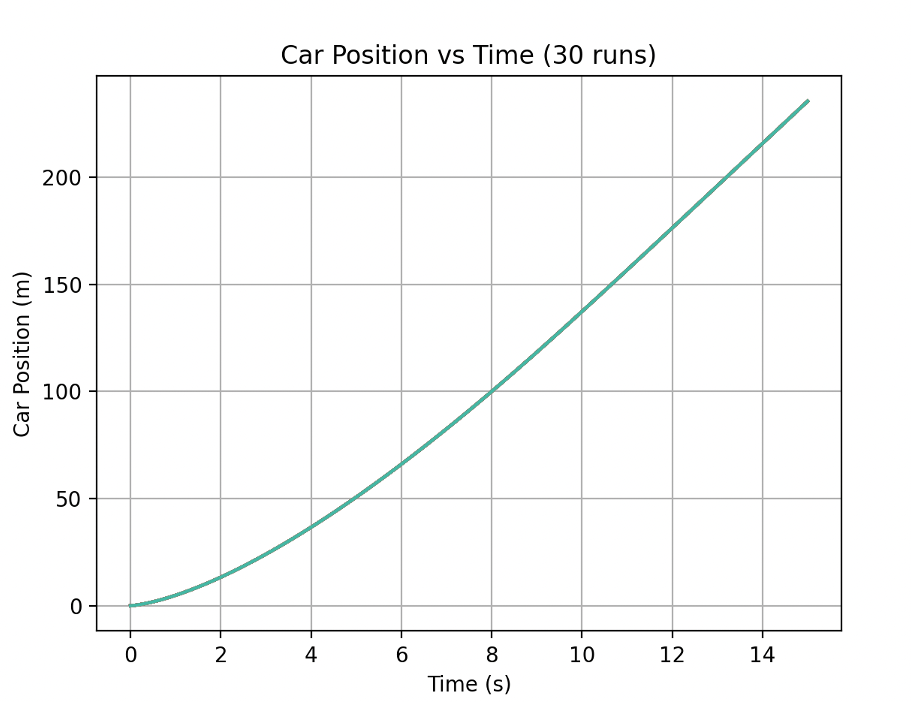
\includegraphics[width=0.5\textwidth]{simulation-figures/car_position_30.png}
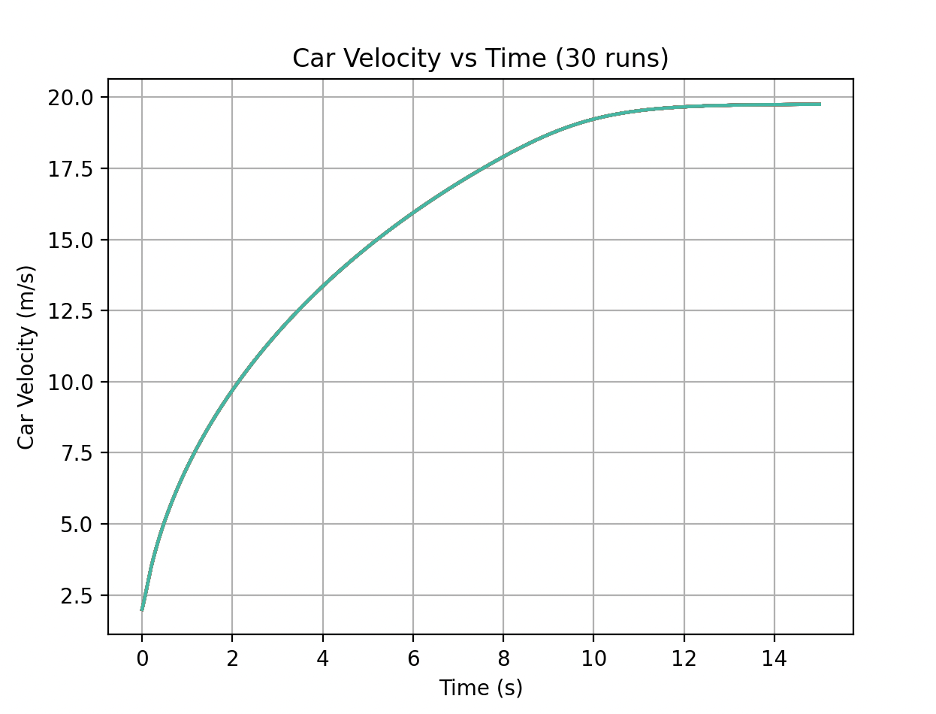
\includegraphics[width=0.5\textwidth]{simulation-figures/car_velocity30.png}
\noindent The graphs above show the Car Position vs Time(Left) and the Car Velocity vs Time(Right) after 30 simulations with the same inputs.
These tests correspond to \textbf{Position test-1} and \textbf{Velocity test-1}. \\
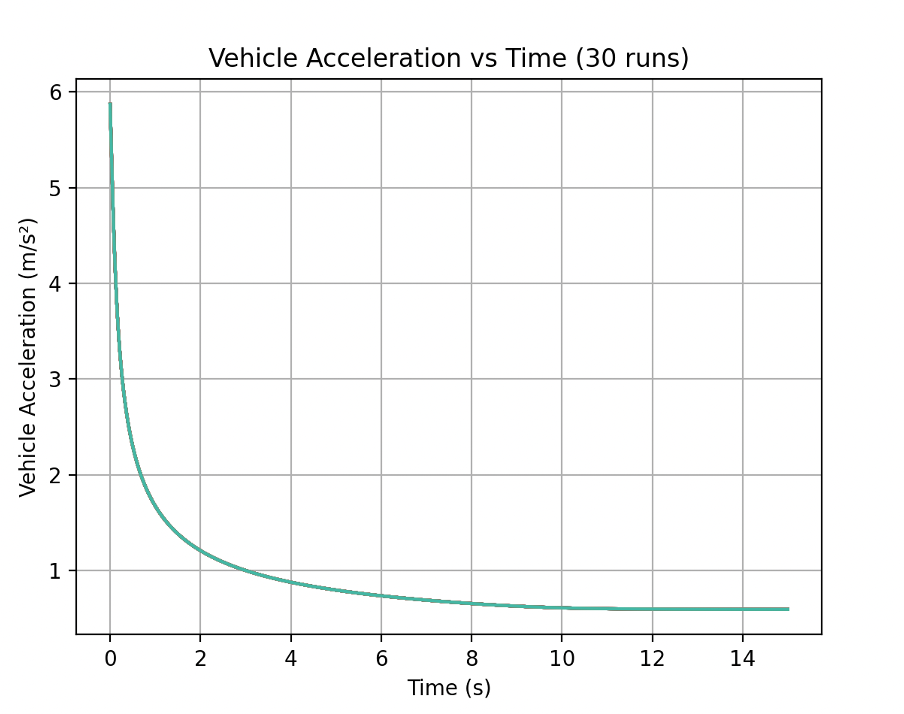
\includegraphics[width=0.5\textwidth]{simulation-figures/vehicle_acceleration30.png}
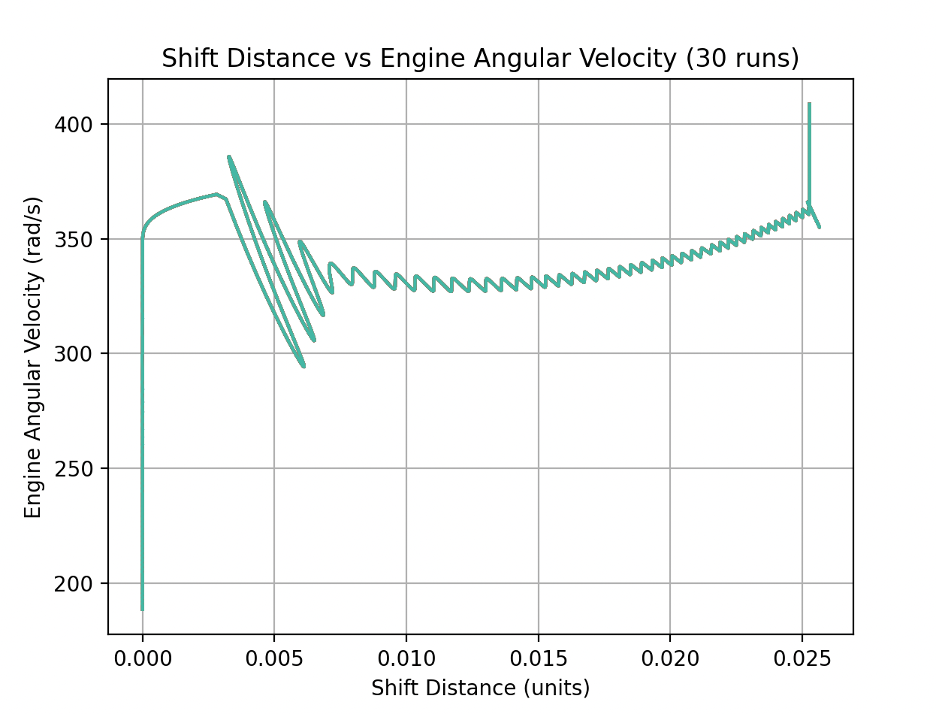
\includegraphics[width=0.5\textwidth]{simulation-figures/shift_distance_vs_engine_velocity30.png}
\noindent The graphs above show the Car Acceleration vs Time(Left) and the Shift Distance vs Engine Angular Velocity(Right) after 30 simulations with the same inputs.
These tests correspond to \textbf{Acceleration test-1} and \textbf{Shift test-1}. \\
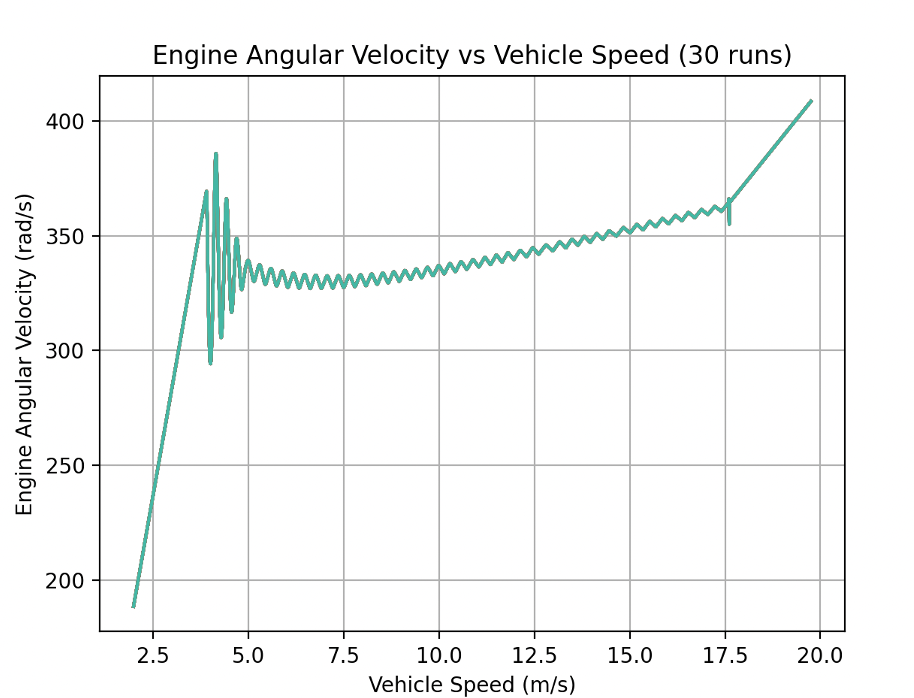
\includegraphics[width=0.5\textwidth]{simulation-figures/shift_curve_30.png}
\\
\noindent The graph above show the Engine Angualr Velocity vs Vehicle Speed. 
These tests correspond to \textbf{Shift test-3} and \textbf{Velocity test-1}. \\
\\
As seen, based on the graphs above, there is little to no variation when performing the tests: \textbf{Position test-1}, \textbf{Velocity test-1}, \textbf{Acceleration test-1}, \textbf{Shift test-1} and \textbf{Shift test-3} 30 times on the same input data.
This passes the test for verifiability. 

\subsection{Understandability}
The Usability/Understandability survey remains in progress at this time and results will be discussed in the \href{file:../UsabilityReport/UsabilityReport.pdf}{Usability Report}. 
Therefore, Understandability test-1 and Understandability test-2 have not been completed yet, however as they are in progress these tests will completed as future work. 

\begin{enumerate}
  \item{\textbf{Understandability test-1}}\\
  Survey question: For the following main features: Inputting parameters, Adjusting parameters, Viewing data outputs, Saving and exporting data. 
  Was the purpose of each function clear, on a scale of 1-5 with 1 being very unclear and 5 being extremely clear. 
  \item{\textbf{Understandability test-2}: Understanding Simulation Outputs}\\
  Survey question: On a scale of 1-5, with 1 being very unclear and 5 being extremely clear, how well did you understand the simulation results and output?
\end{enumerate}

\subsection{Reusability}

The reusability tests are designed to assess how easily the system can be adapted to new or modified configurations. 
\begin{enumerate}
    \item {\textbf{Reusability test-1}}\\
    This test was manually performed by the teams, where the time taken and number of lines of code modified were recorded when implementing the 2023 CVT configuration. 
    Implementation of the 2023 CVT parameters requires at most 20 minutes and involves modifications to approximately 26 lines of code in the \texttt{car\_specs.py} file. 
    These minimal changes demonstrate the system's high reusability, as it can be quickly adapted to new CVT configurations with little effort and modification.
\end{enumerate}
	
\section{Comparison to Existing Implementation}	

Not applicable for this project.
\section{Unit Testing}

\subsection{Back End Unit Testing}
The back end was fully covered by unit tests except for a several files which were not suited for unit testing as they were mainly constants or did not provide functionality that could be tested. \\
\\
The test structure that was created was to essentially mirror how the codebase is organized. There is a test folder which houses all the tests, then inside that there is a simulations and utils folder which contain mirrored test files of the actual files under src/simulations or src/utils.\\
\\
The tests were written using the built-in unittest module in python. The tests were run using the command coverage run -m unittest discover -s test/simulations -s test/utils. This command runs all the tests in those two folders using the coverage library.\\
\\
A coverage report was generated using the command coverage report -m.\\
\\
This command generates a report that shows the percentage of code that was covered by the tests. The report also shows which lines were not covered by the tests.
This can be seen in section 11 of this document.\\

\noindent The following is the file breakdown for the backend unit tests within test/simulations directory:
\\
\texttt{test\_belt\_simulator.py} - This test suite verifies that the BeltSimulator’s methods correctly compute centrifugal force, clamping-derived radial forces, net radial force, slack tension, and maximum transferable torque according to theoretical models.
\\
\texttt{test\_car\_simulator.py} - This test verifies that CarSimulator calculates acceleration correctly as force divided by mass.
\\
\texttt{test\_engine\_simulation.py} - This test suite verifies that EngineSimulator correctly initializes and computes torque, power, and angular acceleration using a mock torque curve.
\\
\texttt{test\_load\_simulation.py} - This test suite verifies that the LoadSimulator correctly computes vehicle load forces (incline, drag, total, gearbox) and acceleration given specific parameters.
\\
\texttt{test\_primary\_pulley.py} - This test suite verifies that the PrimaryPulley class correctly computes flyweight force, spring compression force, net force, and properly handles shift distance limits.
\\
\texttt{test\_secondary\_pulley.py} - This test suite verifies that the SecondaryPulley correctly computes helix force, spring compression force, spring torsion torque, and net force based on theoretical models and geometric parameters. 
\\

\noindent The following is the file breakdown for the backend unit tests within test/utils directory:
\\
\texttt{test\_argument\_parser.py} -- This test suite verifies that \texttt{get\_arguments} correctly parses command line inputs into an object for both default and custom scenarios.
\\
\texttt{test\_conversions.py} - This test suite verifies that conversion functions for angular velocity, angle measurements, circumference, and inch-to-meter conversions return correct values.
\\
\texttt{test\_simulation\_result.py} - This test suite verifies that simulation result correctly parses ODE solutions into system state objects, writes the results to a CSV file, and calls the plot method as expected.
\\
\texttt{test\_system\_state.py} - This test suite verifies that the SystemState class initializes correctly and accurately converts to and from array representations.
\\
\texttt{test\_theoretical\_models.py} - This test suite verifies that Theoretical Models correctly compute various physics and geometry calculations—including Hooke's law, centrifugal force, air resistance, torque, gearing, friction, capstan equation, Newton's second law, and CVT and wrap angle parameters.

\subsection{Front End Unit Testing}
The front end communication protocol was fully covered by unit tests besides the function that calls the python script since it is dependent on the back end Implementation.
\\
The tests are stored in a separate project within the front end solution. They are written using the MS Unit Testing Framework and are run using the dotnet test command.
\\
A coverage report was generated using the JetBrains dotCover tool which shows the percentage of code that was covered by the tests.  

\section{Changes Due to Testing}

\wss{This section should highlight how feedback from the users and from 
the supervisor (when one exists) shaped the final product.  In particular 
the feedback from the Rev 0 demo to the supervisor (or to potential users) 
should be highlighted.}

\subsection{Front End Changes}
On the front end, many changes were made to support unit testing. The communication protocol was separated from the main Unity project since Unity was not compatible with the MS Unit Testing Framework.
\\
Moving the communication protocol into a separate project allowed for the simplification of the code base by isolating responsibilities and improving modularization.
\\
There were also changes on the front end to support the requested changes from the Rev 0 demo. The input parameters were updated to be stored in a csv file and read from there.
\\
These changes were to facilitate the implementation of uploading and downloading the parameters from the front end which was a requested feature from the Rev 0 demo.

\section{Automated Testing}
Both back and front end sets of unit tests were automated and added to the CI/CD pipeline. Now whenever there is a commit it must pass all the tess in order to be verified.
If there is an error it will fail and state which tests failed. This is a good way to ensure that the code is always working as expected.\\
\\
As well the back end coverage report is also generated in the CI/CD run so you can see how much of the code is being covered by tests at that moment.
\\
The configuration for the CI/CD can be seen here: \url{https://github.com/gr812b/CVT-Simulator/blob/develop/.github/workflows/ci.yaml}
\section{Trace to Requirements}

\begin{table}[H]
  \centering
    \begin{tabular}{|c|c|}
      \hline
      \textbf{Requirement} & \textbf{Test(s)} \\ \hline
      R1 & Position test-2, Velocity test-2, Acceleration test-2, Shift test-4  \\ \hline
      R2 & Acceleration test-1, Unit Tests-\texttt{test\_car\_simulator.py} \\ \hline
      R3 & Velocity test-1 \\ \hline
      R4 & Position test-1 \\ \hline
      R5 & Clamping forces test-1, Unit Tests-\texttt{test\_primary\_pulley.py} \\ \hline
      R6 & Clamping forces test-1, Unit Tests-\texttt{test\_secondary\_pulley.py} \\ \hline
      R7 & Shift test-1, Shift test-2, Shift test-3 \\ \hline
      R8 & Shift test-1, Shift test-2, Shift test-3, \texttt{test\_belt\_simulator.py}  \\ \hline
      R9 & Engine test-1, Unit Tests-\texttt{test\_engine\_simulation.py} \\ \hline
      R10 & User Interface test-1, Unit Tests-\texttt{test\_argument\_parser.py}  \\ \hline
      R11 & User Interface test-1, \\ \hline
      R12 & User Interface test-2 \\ \hline
      R13 & User Interface test-3 \\ \hline
      R14 & User Interface test-4 \\ \hline
      R15 & Compatibility test-1 \\ \hline
      R16 & Compatibility test-1 \\ \hline
      \end{tabular}
      \caption{System Functional Requirements and Corresponding Tests}
      \label{tab:requirements_tests}
  \end{table}

  \begin{table}[h!]
    \centering
      \begin{tabular}{|c|c|}
        \hline
        \textbf{Requirement} & \textbf{Test(s)} \\ \hline
        NFR1 & Accuracy test-1  \\ \hline
        NFR2 & Useability test-1, Useability test-2 \\ \hline
        NFR3 & Maintainability test-1 \\ \hline
        NFR4 & Verifiability test-1 \\ \hline
        NFR5 & Understandability test-1, Understandability test-2 \\ \hline
        NFR6 & Reusability test-1 \\ \hline
        \end{tabular}
        \caption{System Nonfunctional Requirements and Corresponding Tests}
        \label{tab:requirements_tests}
    \end{table}
		
\section{Trace to Modules}		

\section{Code Coverage Metrics}

\begin{figure}[H]
  \begin{center}
   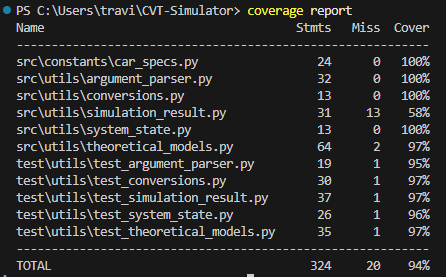
\includegraphics[width=0.7\textwidth]{UnitTestCoverageReport.png}
  \caption{Back End Code Coverage}
  \label{Fig_Home} 
  \end{center}
\end{figure}

\begin{figure}[H]
  \begin{center}
   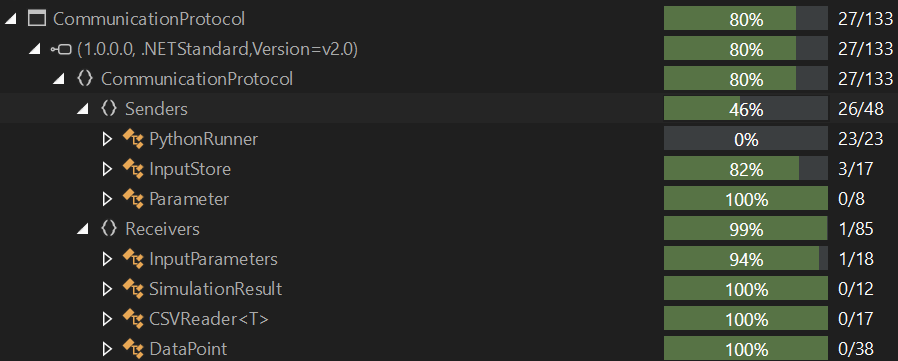
\includegraphics[width=0.7\textwidth]{CSUnitTestCoverage.png}
  \caption{Front End Code Coverage}
  \label{Fig_Home} 
  \end{center}
\end{figure}


\bibliographystyle{plainnat}
\bibliography{../../refs/References}

\newpage{}
\section*{Appendix --- Reflection}

The information in this section will be used to evaluate the team members on the
graduate attribute of Reflection.

\input{../Reflection.tex}

\begin{enumerate}
  \item What went well while writing this deliverable?
  \\
  \\
  Creating the unit tests for the back end was relatively simple as the code was already structured in a way that made it easy to unit test.
  The process of creating the test just involved going through each function and comparing the expected output to the actual output.
  \item What pain points did you experience during this deliverable, and how
    did you resolve them?
  \\
  \\
  Getting front end unit testing to work was a challenge since Unity was not compatible with many unit testing frameworks.
  The solution was to separate the communication protocol into its own project which then allowed us to use the MS Unit Testing Framework.
  This also allowed us to simplify the code base by isolating responsibilities and improving modularization.
  \item Which parts of this document stemmed from speaking to your client(s) or
  a proxy (e.g. your peers)? Which ones were not, and why?
  \item In what ways was the Verification and Validation (VnV) Plan different
  from the activities that were actually conducted for VnV?  If there were
  differences, what changes required the modification in the plan?  Why did
  these changes occur?  Would you be able to anticipate these changes in future
  projects?  If there weren't any differences, how was your team able to clearly
  predict a feasible amount of effort and the right tasks needed to build the
  evidence that demonstrates the required quality?  (It is expected that most
  teams will have had to deviate from their original VnV Plan.)
  \\
  \\
  The back end unit testing was conducted as planned in the VnV Plan while the front end unit testing required modification to our approach.
  On the front end, the Unity Testing Framework was significantly less user friendly and comprehensive than we expected.
  This required us to change our approach to unit testing on the front end and move towards our current solution.
  This was not anticipated in the VnV Plan as we were not aware of the limitations of the Unity Testing Framework.
  In future projects, we would be able to better anticipate these changes by doing more research on the tools we plan to use.
  On the back end, we were able to correctly predict the amount of effort and the tasks needed based on our previous experience with unit testing.
  The back end unit testing followed the standard procedure and was able to easily leverage existing packages and tools to support the testing.
\end{enumerate}

\end{document}